% Author: Bernard Lampe

% Use the IEEE classes
\documentclass[journal]{IEEEtran}

% Packages
\usepackage[cmex10]{amsmath}
\usepackage{url}
\usepackage{cite}
\usepackage{graphicx}
\usepackage{subfig}
\usepackage{float}

% Correct bad hyphenation here
\hyphenation{op-tical net-works semi-conduc-tor}

% Start document
\begin{document}

% Paper title
\title{Computation of Channel Capacity}

% Author
\author{Bernard~Lampe,~\IEEEmembership{Member,~IEEE}}

% The paper headers
\markboth{Computation of Channel Capacity}%
{Shell \MakeLowercase{\Lampe}: Computation of Channel Capacity}

% Make the title area
\maketitle

\begin{abstract}
The maximum capacity of a discrete memoryless channel can be computed as a solution to a convex optimization problem. An efficient algorithm for numerically solving for the capacity of a channel was developed by Blahut. Blahut's algorithm exploits the convex structure of the problem by formulating an iterative set of equations which converges on the optimal solution. In this paper we demonstrate Blahut's algorithm by computing the channel capacities of discrete \(n^{th}\) binary channel of varying sizes. Then we observe the changes in channel capacity as the number of input and output symbols varies.
\end{abstract}

% Keywords
\begin{IEEEkeywords}
Blahut, Channel Capacity, Binary Channel
\end{IEEEkeywords}

% Introduction with drop letter and first word capitalized.
\section{Introduction}
\IEEEPARstart{C}{hannels} are fundamental abstract representations of a communication process. They are useful for mathematically modeling the characteristics of a particular communication. If an entity \begin{math}A\end{math} communicates with entity \begin{math}B\end{math}, \begin{math}A\end{math} will physically act to transfer information via an avaliable transport medium. A successful transfer of information occurs when \begin{math}A\end{math} and \begin{math}B\end{math} agree on what has been sent. The entity \begin{math}A\end{math} is able to send any arbitrary set and sequence of symbols desired. However, if \begin{math}A\end{math} does send information arbitrarily in a noisy channel, then a particular observed output may have resulted from multiple inputs. In effect the receiving entity, \begin{math}B\end{math}, is unable to determine what was sent and information is lost. If the sending party reduces the symbols being sent to a subset of those available, a scheme can be devised which will prevent ambiguity on the output of the channel. By imposing such a scheme the rate at which \begin{math}A\end{math} is sending signals is reduced. However, the confusion of the recieving party is also reduced. The act of designing such a scheme is known as coding. Claude Shannon was the first to discover that for any channel, there is a maximum rate at which you can unambiguously send information. The maximum rate is known as the channel capacity and is defined as the maximum of the mutual information between the input and output over all possible distributions of the input. \cite[p.~183-184]{cover}.

\par This analysis will discuss discrete memoryless channels. A channel is memoryless if any particular received output symbols is only dependent upon the input which was induced. A formal description of a discrete channel consists of a set of input symbols \begin{math}X = \{x_j\}, j = {0, 1,\dots, m}\end{math}, and set of output symbols \begin{math}Y = \{y_k\}, k = {0, 1,\dots, n}\end{math} and a probability transition matrix \begin{math}Q_{k|j}\end{math} as shown in equation \ref{eq:transitionMatrix}. The transition matrix specifies the probability of receiving any particular output symbol when given an input symbol. Throughout the remainder of the paper, we may refer to individual transition probabilities as \begin{math}p(k|j) = p(y_k|x_j)\end{math}. This means the probability of receiving symbol \begin{math}y_k\end{math} when symbol \begin{math}x_j\end{math} was sent.

\begin{equation}
\label{eq:transitionMatrix}
Q_{k|j} = \begin{pmatrix}
p(y_0|x_0) & p(y_1|x_0) & \dots & p(y_n|x_0) \\
p(y_0|x_1) & p(y_1|x_1) & \dots & p(y_n|x_1) \\
\vdots & \vdots &  \ddots & \vdots \\
p(y_0|x_m) & p(y_1|j_m) & \dots & p(k_n|j_m) \end{pmatrix}
\end{equation}

\par For a discrete memoryless channel, Claude Shannon defined the channel capacity as the maximum of the mutual information between the input and output as in equation \ref{eq:maxI}. This maximization is taken over all input probability distributions. Shannon also showed that this particular function is concave over a closed convex set \cite{shannon}. Therefore, it could be solved using a simple gradient search or Blahut's iterative algorithm which we are exhibiting here \cite[p.~191]{cover}.

\begin{equation}
\label{eq:maxI}
C = \max_{p(x_j)}I(X;Y)
\end{equation}
\begin{equation}
p(x_j) \geq 0, \forall j \text{ and } \sum_{j=0}^{m}p(x_j) = 1
\end{equation}

\par The mutual information between the input and output, expressed in bits, is defined by Shannon as in equation \ref{eq:mutualInfo}. Shannon proved the existence of an optimal distribution of the input symbols \begin{math}p(x_j)\end{math} which could achieve the channel capacity. The proof is non-constructive, but Blahut composed an algorithm that computes the optimal distribution by taking advantage of the convex nature of the problem. His algorithm begins with a guess of the input distribution \(p(x_j)\) and numerically iterates until the distribution represent the maximum mutual information \(I(X;Y)\) \cite{blahut}.

\begin{equation}
\label{eq:mutualInfo}
I(X;Y) = \sum_{k=0}^{n}\sum_{j=0}^{m}p(y_k|x_j)p(x_j)log_{2}\left(\frac{p(y_k|x_j)}{\sum_{j=0}^{m}p(y_k|x_j)p(x_j)}\right)
\end{equation}

% Describe Blahut's Algorithm
\subsection{Blahut's Algorithm}
\par Blahut's algorithm is an iterative solution to the equation \ref{eq:maxI}. The algorithm takes advantage of the concave nature of the definition of mutual information. Mutual information is a concave function over any choice of \begin{math}p(x_j)\end{math} for the input distribution. Therefore, the equation can be casted as a convex optimization. Blahut constructed an iterative mapping from one probability distribution to another which will monotonically converge on the maximum of the concave mutual information function. Given a single input and output entity, this maximum is the global maximum mutual information and subsequently the channel capacity \cite{blahut}.
\par Blahut's algorithm begins by choosing a starting probability distribution at iteration \begin{math}r = 0\end{math} as in equation \ref{eq:beginP}. In practice, choosing a uniform distribution at iteration \begin{math}r = 0\end{math} works well. The mapping formulated by Blahut computes the next iteration \begin{math} r+1 \end{math} of the probability distribution via equations \ref{eq:computec} and \ref{eq:iter} \cite{blahut}.

\begin{equation}
\label{eq:beginP}
p(x_j)^r \geq 0, \forall j \text{ and } \sum_{j=0}^{m}p(x_j)^r = 1
\end{equation}

\begin{equation}
\label{eq:computec}
c(x_j)^r = exp\left(\sum_{k=0}^{n}Q_{k|j} log_2\left(\frac{Q_{k|j}}{\sum_{j=0}^{m}p(x_j)^rQ_{k|j}}\right)\right)
\end{equation}

\begin{equation}
\label{eq:iter}
p(x_j)^{r+1} = p(x_j)^r\frac{c(x_j)^r}{\sum_{j=0}^{m}p(x_j)^rc(x_j)^r}
\end{equation}

\par Blahut also formulated stopping criteria by specifying an equation which determines the amount of convergence and channel capacity at each iteration \begin{math}r\end{math}. The formulation relies on the inequality in equation \ref{eq:uplow}. The stopping criterion for the algorithm occurs when the difference between the upper and low bound of \begin{math}C^r\end{math} becomes smaller than a predefined epsilon \begin{math}\epsilon\end{math} as in equation \ref{eq:stop}. Upon convergence the channel capacity is computed as the lower bound of equation \ref{eq:uplow} as in equation \ref{eq:finalc} \cite{blahut}.

\begin{equation}
\label{eq:uplow}
log_2\left(\sum_{j = 0}^{m}p(x_j)^rc(x_j)^r\right) \leq C^r \leq log_2(\max_j c(x_j)^r)
\end{equation}

\begin{equation}
\label{eq:stop}
log_2(\max_j c(x_j)^r) - log_2\left(\sum_{j = 0}^{m}p(x_j)^rc(x_j)^r\right) < \epsilon
\end{equation}

\begin{equation}
\label{eq:finalc}
C = \max_{p(x_j)}I(X;Y) = log_2\left(\sum_{j = 0}^{m}p(x_j)^rc(x_j)^r\right)
\end{equation}

% Show results on binary erasure channel
\subsection{Binary Erasure Channel Capacity}
\par We implemented Blahut's algorithm using matlab. Also, we validated the algorithm performance by computing the channel capacity of the simple binary erasure channel. The channel capacity of such a simple channel can be computed analytically and therefore makes a good candidate for validation of the algorithm. A depiction of the simple channel is in figure \ref{im:erasure}. This simple channel models a communication channel in which bits could be lost (erased) during transmission with probability \begin{math}\alpha\end{math}. It has been analytically shown that the capacity of this channel is \begin{math}C = 1-\alpha\end{math} and the optimal distribution of the input is achieve with \begin{math}p(x_0) = p(x_1) = \frac{1}{2}\end{math} \cite[p.~88-189]{cover}.

\begin{figure}[h]
\centering
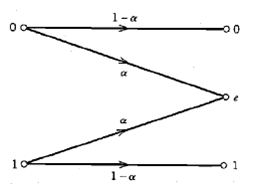
\includegraphics[width=2in]{../images/binaryErasureChannel.png}
\caption{Binary Erasure Channel}
\label{im:erasure}
\end{figure}

\par The transition matrix for the binary erasure channel is in equation \ref{eq:binTran}. There are two rows representing the input symbols (bits) and three columns representing the output symbols (bits or erased). For verification we defined \begin{math}\alpha = 0.2\end{math}, and the matlab implementation computed the \begin{math}C = 1 - \alpha = 0.8\end{math} and the input distribution which maximized the channel capacity as \begin{math}p(x_0) = p(x_1) = 0.5\end{math}. This result gives evidence of the correctness of implementation. Other parameters and transition matrices were tested, and all validated the correctness of the code.

\begin{equation}
\label{eq:binTran}
Q_{k|j} = 
\begin{pmatrix}
1-\alpha & \alpha & 0 \\
0 & \alpha & 1-\alpha
\end{pmatrix}
\end{equation}

\section{Experiments}
\subsection{\(N^{th}\) Binary Channel Capacity}
\par With the validated matlab implementation of Blahut's algorithm, we explore the channel capacity of a \(n^{th}\) binary channel of varying sizes. The channel is defined by two positive integers, \(m\) and \(n\). The channel transition matrix is specified by \(Q_{k|j} = \{p(k|j)\}_{j=0,k=0}^{m,n}\). The values of \(p(k|j)\) are give by equation \ref{eq:bintran} where \(j = 0,\dots,m\) and \(k = 0,\dots,n\).

\begin{equation}
\label{eq:bintran}
p(k|j) = {n \choose k} \left(\frac{j}{m}\right)^k \left(1-\frac{j}{m}\right)^{n-k}
\end{equation}

\par The channel defined by \ref{eq:bintran} is called a generalized \(n^{th}\) binary channel because the channel matrix is characterized by a binomial distribution with \(n\) coin flipping trials. Note that the described channel is of dimensions \(m+1\) inputs and \(n+1\) outputs. We will be computing the channel capacities \(C_{m+1,n+1}\) for channels of dimensions where \(m=10,20,30,40,50\) and \(n=10,20,30,40,50\). If we graph the transition matrix for a channel of size \( (m,n) = (50,50) \), as in figure \ref{fig:nthbinplot}, we see that most of the transition probability is concentrated in the matrix diagonal. In addition, the transition probability at the diagonal extremes is one. Therefore, in this channel, it is possible to send the symbol \(x_0\) and \(x_{50}\) without error. However, other symbols may be subject to error during transmission.

\begin{figure}[h]
\centering
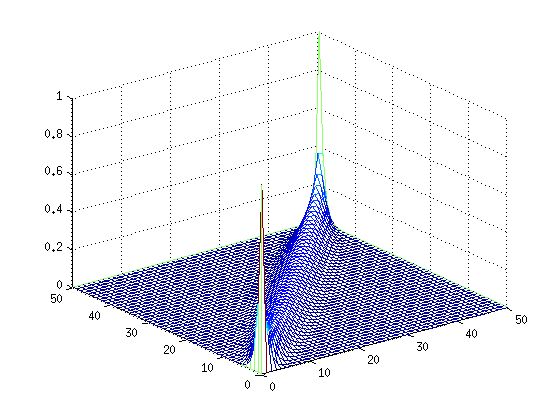
\includegraphics[width=3.1in]{../images/nthBinaryChannel.png}
\caption{Transition Matrix of \(n^{th}\) Binary Channel}
\label{fig:nthbinplot}
\end{figure}

\subsection{Analysis of \(N^{th}\) Binary Channel Capacities}
\par The channel capacities were computed, in bits, for varying sizes of the \(n^{th}\) binary channel. The results are below in table \ref{tab:capacities}. By analyzing the table of capacities, two obvious trends appear.

\begin{table}[h]
\normalsize
\caption{\(N^{th}\) Binary Channel Capacities}
\label{tab:capacities}
\begin{tabular}{|c|c|c|c|c|c|}
\hline
& \(n = 10\) & \(n = 20\) & \(n = 30\) & \(n = 40\) & \(n = 50\) \\
\hline
\(m = 10\) & 1.7771  &  2.1397  &  2.3636  &  2.5054  &  2.6051 \\
\hline
\(m = 20\) & 1.7774  &  2.1401  &  2.3672  &  2.5371  &  2.6719 \\
\hline
\(m = 30\) & 1.7776  &  2.1405  &  2.3689  &  2.5372  &  2.6701 \\
\hline
\(m = 40\) & 1.7777  &  2.1407  &  2.3695  &  2.5375  &  2.6720 \\
\hline
\(m = 50\) & 1.7777  &  2.1408  &  2.3695  &  2.5382  &  2.6715 \\
\hline
\end{tabular}
\end{table}

\par The first is seen when examining the columns of  of the data. When the number of output symbols remains constant, the capacity of the channel does not increase significantly when the number of input symbols is increased. For example, the difference between the channel capcities when the number of inputs is \(m = 10\) and \(m = 50\), but the number of outputs remains the same \(n = 50\) is only \(0.0664\) bits.
\par The second trend is observed when examining the rows of the data. When the number of input symbols is constant, and the number of output symbols increases, the channel capacity increase considerably. If we plot the rows of the channel capcity matrix in table \ref{tab:capacities}, we see a logrithmic increase in the channel capacities as the number of output symbols increases. The plot is in figure \ref{fig:graph}.

\begin{figure}[h]
\centering
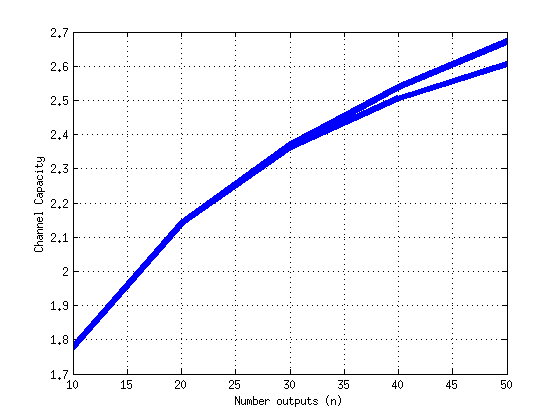
\includegraphics[width=3.1in]{../images/graph.png}
\caption{Channel Capacities as \(n\) Increases}
\label{fig:graph}
\end{figure}

\par Given the observations made above, it is intuitively clear that the number of output symbols is the limiting factor in this channel. A channel characterized by equation \ref{eq:bintran} appears to be ``output limited'' in that the number of output symbols is the dominating factor in the channel capacity. If you examine the transition matrix in figure \ref{fig:nthbinplot} you will notice that one particular input symbol can map probabilistically to a narrow range of adjacent output symbols with the maximum probability density for a particular symbol being on the correct output symbols. Therefore, increasing the number of output symbols results in an input symbol being mapped unambiguously to a unique range of output symbols (i.e. the output symbols ranges do not overlap). Therefore, to increase the channel capacity, the number of output symbols must be increased such that every input symbols has a range of output symbols in which to map. Thereby giving each input symbols it's own unique range of adjacent output symbols so that the receiving entity can determine what has been sent. However, there are diminishing returns in that increasing the number of output symbols results in a logrithm increase of the channel capacity.

\section{Conclusion}
\par In this paper we have briefly explained the general definition of a channel as characterized by Claude Shannon. In addition, we have detailed Blahut's iterative algorithm for computing the channel capacity and optimizing input probability distribution for a particular channel. We implemented the algorithm in matlab and verified the code using simple channels which have analytically tractable solutions. Finally, we described a \(N^{th}\) binary channel and computed channel capacities for a range of channels sizes. Through analysis of these capacities, it was observed that the capacity of the \(n^{th}\) binary channel is increasing when the number of output symbols increases. It was also observed that the capacity is not significantly increased with an increasing number of input symbols. This leads to the conclusion that this particular type of channel is ``output limited''.

% References section
\nocite{*}
\bibliographystyle{plain}
\bibliography{./references}

% Biography
\begin{IEEEbiographynophoto}{Bernard Lampe}
(M'09) became an IEEE Member (M) in 2009 and received his bachelors of science degree from The University of Michigan in Ann Arbor, Michigan, USA in 2009.
\par Mr. Lampe is also a member of the American Society for Computing Machines (ACM) since 2009.
\end{IEEEbiographynophoto}

% End document
\end{document}

